\clearpage
\section*{Task 4 - Point Processing}

\subsection*{Intensity transform}

The gamma correction is done by applying the function $px_{new} = {px_{old}}^{\gamma}$.
Because we're operating with input and output that is integers in the [0, 255] range, not floating point numbers in the [0, 1] range, we need to take this into consideration for the calculation.
\begin{lstlisting}[language=Python, label=gamma_correction, caption=Gamma correction]
def pixel_wise_transform(matrix, fun):
    '''
    applies fun(px) to every px in the 2d matrix
    '''
    return np.asarray(map(lambda row: map(lambda px: fun(px), row), matrix))


def gamma_correct(matrix, gamma=1.0):
    '''
    applies the gamma correction function (px)^(gamma) to the matrix
    '''
    return pixel_wise_transform(matrix, lambda px: int(255 * ((px / 255) ** gamma)))
\end{lstlisting}

\begin{figure}[h!]
    \centering
    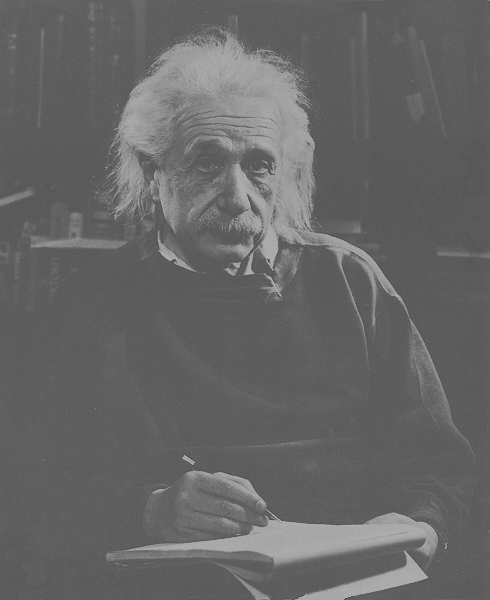
\includegraphics[width=5cm]{../LAB1/img/einstein_lowcontrast.png}
    \includegraphics[width=5cm]{../LAB1/output/gamma_einstein_lowcontrast.png}
    \includegraphics[width=5cm]{../LAB1/output/stretched_gamma_einstein_lowcontrast.png}
    \caption{From the left: einstein\_lowcontrast.png, gamma corrected, input range stretched then gamma corrected.}
\end{figure}


\begin{lstlisting}[language=Python, label=input_range, caption=Input range stretching]
def minmax_2d(matrix):
    '''
    returns the minimum and maximum value of a 2d matrix
    '''
    return map(lambda f: f(f(matrix, key=lambda x: f(x))), (min, max))


def stretch_range(matrix):
    '''
    stretches the range of matrix to [0, 255]
    '''
    m_min, m_max = minmax_2d(matrix)
    return pixel_wise_transform(matrix, lambda px: int((px - m_min) / ((m_max - m_min) / 255)))
\end{lstlisting}

\subsection*{Histogram equalization}
